\part{Databases}

\chapter{Основные понятия}

\section{Теорема CAP}

Теорема CAP (известная также как теорема Брюера) — эвристическое утверждение о том, что в любой реализации распределённых вычислений возможно обеспечить не более двух из трёх следующих свойств:
\begin{itemize}

\item согласованность данных (англ. consistency) — во всех вычислительных узлах в один момент времени данные не противоречат друг другу;
\item доступность (англ. availability) — любой запрос к распределённой системе завершается корректным откликом, однако без гарантии, что ответы всех узлов системы совпадают;
\item устойчивость к разделению (англ. partition tolerance) — расщепление распределённой системы на несколько изолированных секций не приводит к некорректности отклика от каждой из секций.

\end{itemize}

\section{Чем отличается транзакция от запроса в контексте БД}
Транзакция - это несколько последовательных запросов в БД, если хотя бы одна из них завершается, то вся транзакция отменяется (rolling back).

\section{Модель транзакции в стандарте ANSI ISO}
\subsection{Что такое ACID}

Atomicity - не делимая операция.
Consistency - арифмитические правила, уголовный кодекс, здравый смысл.
Isolation - независимость друг от друга.
Durability - диск надежное хранилище.

\chapter{Масштабируемость}

\section{Write ahead logging}

\section{Модели согласованности}
Подход, используемый в той или иной распределённой системе (распределённой общей памяти[en], СУБД, файловой системе), для обеспечения гарантий согласованности данных. 

Особую роль для модели согласованности играет вопрос линеаризуемости программы, в которой вместо операций чтения и записи рассматриваются операции над объектами (например функции, процедуры), а состояние памяти в данной модели — это состояния объектов. Линеаризуемые программы применяются для систем с объектной организацией общей памяти. В отличие от всех остальных систем, такие программы не могут напрямую использовать общие переменные (состояние объектов), а только через специальные функции-методы (операции). Для этих систем линеаризуемость совпадает со строгой согласованностью. 

\subsection{Что такое согласованность данных?}

\subsection{Причинная согласованность}
Или causal consistency, - модель согласованности, которая не требует, чтобы все процессы видели одну и ту же последовательность записей в памяти, проводя различие между потенциально-зависимыми (запись одной может зависеть от результата чтения другой ячейки) и потенциально-независимыми (параллельными) операциями записи.

\subsection{строгая согласованность}
\subsection{последовательная согласованность}
\subsection{PRAM-согласованность}
\subsection{процессорная согласованность}
\subsection{слабая согласованность }
\subsection{согласованность в конечном счёте}
\subsection{согласованность по выходу}
\subsection{согласованность по входу}

\section{Алгоритмы разрешения конфликтов при репликации}
\subsection{Quorum}
\subsection{Векторные часы}
\subsection{Часы Лемпорта}

\section{Шардирование}
\section{Блокировки}

\subsection{Оптимистичные и пессимистичные}
\subsection{Блокировки таблицы и отдельных строк}
\subsection{Алгоритм 2-фазного блокирования 2PL}

В базах данных и обработке транзакций двухфазная блокировка (2PL) — это метод управления параллелизмом, который гарантирует сериализуемость[1][2]. Это также имя результирующего набора графиков транзакций базы данных (истории). Протокол использует блокировки, применяемые транзакцией к данным, которые могут блокировать (интерпретировать как сигналы для остановки) другие транзакции от доступа к тем же данным в течение жизни транзакции.

По протоколу 2PL блокировки (locks) применяются и удаляются в два этапа:

Фаза расширения: блокировки берутся и ни одна блокировка не освобождается.

Фаза сокращения: блокировки освобождаются и ни одна блокировка не берётся.

В базовом протоколе используются два типа блокировок: Shared и Exclusive locks. Уточнения базового протокола могут использовать больше типов блокировок. Используя блокировки, блокирующие процессы, 2PL могут подвергаться взаимоблокировкам, которые являются результатом взаимной блокировки двух или более транзакций. 

\subsection{Что такое эскалация блокировок?}

\chapter{Реляционная теория}
\subsection{Что такое транзитивная завивсимость?}
\subsection{Нормальные формы?}
\begin{enumerate}
    \item 1ая;
    \item 2ая;
    \item 3ая;
    \item Бойса-Кодда;
    \item 4ая;
    \item Доменная форма;
    \item 5ая;
    \item 6ая;
\end{enumerate}
\subsection{Ограничение целостности базы данных?}

\chapter{PostgreSQL}

\section{Архитектура posgres}
\subsection{Внутренние компоненты}
\subsection{Что такое autovacuum?}
\subsection{Как данные попадают на диск?}

\begin{figure}[h!]
\centering
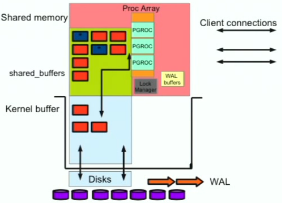
\includegraphics[width=0.8\textwidth]{img/postgres-scheme-buffers.png}
\caption{Схема работы буфферов}
\label{postgres-buffers}
\end{figure}

\section{Что такое план запроса?}

\section{Транзакции}

\subsection{Проблемы параллельного доступа}
\subsubsection{lost update}
\subsubsection{dirty read}
\subsubsection{non-repeatable read}
\subsubsection{phantom reads}

\subsection{Уровни изоляции}
Под «уровнем изоляции транзакций» понимается степень обеспечиваемой внутренними механизмами СУБД (то есть не требующей специального программирования) защиты от всех или некоторых видов вышеперечисленных несогласованности данных, возникающих при параллельном выполнении транзакций. Стандарт SQL-92 определяет шкалу из четырёх уровней изоляции: Read uncommitted, Read committed, Repeatable read, Serializable. Первый из них является самым слабым, последний — самым сильным, каждый последующий включает в себя все предыдущие. 

\subsubsection{Read uncommitted}
\subsubsection{Read committed}
\subsubsection{Repeatable read}
\subsubsection{Serializable}
\subsubsection{Snapshot isolation}

\subsection{Распределенные транзакции}

Дока постгреса:
\href{https://www.postgresql.org/docs/12/sql-prepare-transaction.html}{Postgres doc}

\section{Индексы в postgres}
Индекс - это дополнительная структура данных для ускорения запросов.

Индексы нужны для: поиска, сортировки (WHERE), группировки, ограничения целостности.

\begin{figure}[h!]
\centering
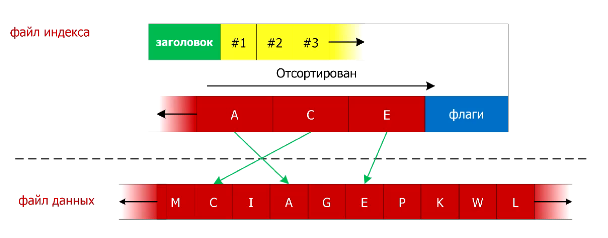
\includegraphics[width=0.8\textwidth]{img/index-sort.png}
\caption{Внешний файл с индексом и ортсортированной колонкой}
\label{index-sort}
\end{figure}

Отрицательные стороны индексов \label{index-usage}:
\begin{itemize}
\item Обладает малой селективностью, пример:
База данных с муж и жен полом, когда статистически записей примерно одинаковое количество.
\item Размер, иногда может весить боьлше базы;
\item Индекс расчитывается в момент вставки записи в таблицу, это занимает время, иногда до 80% времени вставки;
\item Индекс может долго работать, если он большой и фрагментированный;
\item Индекс должен быть валиден во время использования.
\end{itemize}

\subsection{Аспекты создания индекса}

\begin{itemize}
\item Создание без остановки базы:
\begin{python}
CREATE INDEX CONCURRENTLY a\_ind in table (a);
\end{python}
\item Важен порядок полей, кроме GIN:
\begin{python}
SELECT * FROM table WHERE b > 2 AND b IS NOT NULL;
CREATE INDEX a_ind ON table (a,b) WHERE b IS NOT NULL;
\end{python}
Гарантии попадания в индекс нет.
\item План запроса с индексом должен быть оптимален, для построения плана запроса используется cost-base оптимайзер. Строятся всевозможные планы, то как можно достать данные. Вычисляется веса (цены) каждой операции. Выбирается план с минимальной стоимостью.
\end{itemize}

\subsection{Виды проходов по индексу}

\subsubsection{seq scan}
Не использование индекса, бежим по таблице и сравниваем значения, O(n). Подходит для маленьких таблиц, которые скорее всего попадут в page cache.
\subsubsection{index scan}
Выносим колонку в отдельный файл и строим индекс, получаем: файл индекса и файл таблицы. После нахождения индекса нужно сходить в файл с таблицей. Хорошо подходит для разряженных таблиц. Эффективен для раряженных выборок, когда выбираемых значений в базей 20-25%.
\subsubsection{index only-scan}
Читаем только индекс, не обращаясь к диску. Для этого введена карта видимости. Например count() позволяет выполнять такой запрос.
\subsubsection{bitmap index scan}
Мы хотим выполнить запрос WHERE col1 = A AND col2 = B, но у нас нет индекса col1 AND col2, у нас индексы col1, col2. Тогда постгрес тросить битовую карту по каждому из индексов и объединяет их.
Еще используется для оптимизации последовательных чтений диска.

Если в explain запроса появляется FIlter - это означает неполноту покрытия условия индексом 
\subsubsection{index only scan}
\subsubsection{bitmap heap scan}

\subsection{Типы индексов}

\subsubsection{b-tree}
Это сбалансированное дерево.
Используется там, где нужно получить, например, первые 100 записей отсортированные по определенному полю:
\begin{figure}[h!]
\centering
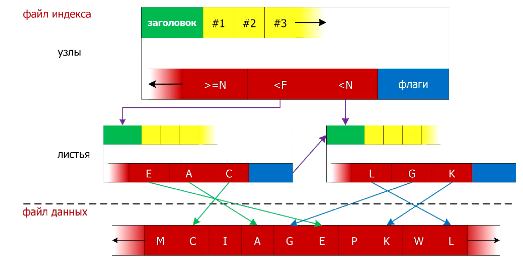
\includegraphics[width=0.8\textwidth]{img/btree.png}
\caption{B-Tree индекс, с оптимизациями}
\label{btree}
\end{figure}

\subsubsection{hash}
\subsubsection{gin}
Полнотекстовый поиск.
\subsubsection{gist}
\subsubsection{sp-gist}
\subsubsection{brin}

\subsubsection{Функциональный индекс}
Можем вынести индекс в функцию. Аспекты:
\begin{itemize}
\item Функция должна быть immutable;
\item Изменение индекса очень дорого;
\item Условие при поиске должно точно совпадать;
\item Функцию можно изменить - но индекс будет не корректный!
\end{itemize}

Пример построения индекса по функции:
\begin{python}
CREATE OR REPLACE FUNCTION foo(text)
RETURNS test AS $$ RERURN replace(test, 'e', 'r');
$$
LANGUAGE sql IMMUTABLE COST 1;
\end{python}
Использование:
\begin{python}
CREATE INDEX ind_a ON table USING btree (foo(name));
\end{python}

\section{Мониторинг индексов}
\begin{itemize}
\item Неиспользуемые индексы
\item Дублирующие индексы
\end{itemize}

\href{https://wiki.postgresql.org/wiki/Index_Maintenance}{Indexes}

\section{Что такое include индексы?}
\section{Как посмотреть индексы для таблицы?}
\section{Всегда ли postgres использует индексы?}
Нет, см. \S \ref{index-usage}.

\section{Обеспечение надежности}
\subsection{Что такое WAL?}
Журнал предзаписи (WAL) — это стандартный метод обеспечения целостности данных. Детальное описание можно найти в большинстве книг (если не во всех) по обработке транзакций. Вкратце, основная идея WAL состоит в том, что изменения в файлах с данными (где находятся таблицы и индексы) должны записываться только после того, как эти изменения были занесены в журнал, т. е. после того как записи журнала, описывающие данные изменения, будут сохранены на постоянное устройство хранения. Если следовать этой процедуре, то записывать страницы данных на диск после подтверждения каждой транзакции нет необходимости, потому что мы знаем, что если случится сбой, то у нас будет возможность восстановить базу данных с помощью журнала: любые изменения, которые не были применены к страницам с данными, могут быть воссозданы из записей журнала. (Это называется восстановлением с воспроизведением, или REDO.)


\chapter{Redis}

\section{Есть ли транзакция в Redis?}
\section{Типы данных Redis}
\subsection{Строки (strings)}
Базовый тип данных Redis. Строки в Redis бинарно-безопасны, могут использоваться так же как числа, ограничены размером 512 Мб.
\subsection{Списки (lists)}
Классические списки строк, упорядоченные в порядке вставки, которая возможна как со стороны головы, так и со стороны хвоста списка. Максимальное количество элементов - 232 - 1.
\subsection{Множества (sets)}    
Множества строк в математическом понимании: не упорядочены, поддерживают операции вставки, проверки вхождения элемента, пересечения и разницы множеств. Максимальное количество элементов - 232 - 1.
\subsection{Хеш-таблицы (hashes)}    
Классические хеш-таблицы или ассоциативные массивы. Максимальное количество пар «ключ-значение» - 232 - 1.
\subsection{Упорядоченные множества (sorted sets)}
Упорядоченное множество отличается от обычного тем, что его элементы упорядочены по особому параметру «score».
